Gravitational waves provide valuable insight into the formation and physics of compact objects. It is important to accurately detect and measure their parameters, specifically eccentricity in our case. In this chapter we review existing literature that underlies the results of this thesis. First, we describe eccentricity and the derivation of equations describing the decrease in energy, angular momentum, semimajor axis, and eccentricity due to gravitational radiation. Next, we describe the methods and algorithms used to detect gravitational-waves and determine their significance. Finally, we describe the Bayesian methods and algorithms used to measure the parameters of detected gravitational-wave signals.

\section{Gravitational Waves from Eccentric Binary Inspiral}\label{GW-eccentricity} 

Circular binary systems that consist of two neutron stars with mass $m_1$, $m_2$, separated by a distance, d with eccentricity, $e = 0$ have been considered in Refs.~\cite{misner:1973,Brown:2004vh}. Here we consider a similar case with non-zero eccentricity, $e \neq 0$. Eccentricity describes how much an object's orbit deviates from a circle. As gravitational radiation is emitted, there is a loss of energy and angular momentum. However, unlike in the circular case, in the case of non-zero eccentricity as gravitational waves are emitted there is a decrease in the eccentricity and semi-major axis.

In 1918, Albert Einstein derived formula that described gravitational radiation, known as the quadrupole formula, which are written as \cite{misner:1973,Peters:1963ux,Peters:1964zz}

\begin{equation}\label{dEdt}
    \frac{dE}{dt} = -\frac{G}{5c^5}\left(\frac{d^3Q^{TT}_{ij}}{dt^3}\frac{d^3Q^{TT}_{ij}}{dt^3} - \frac{1}{3}\frac{d^3Q^{TT}_{ii}}{dt^3}\frac{d^3Q^{TT}_{jj}}{dt^3}\right),
\end{equation}

\begin{equation}\label{dLdt}
    \frac{dL}{dt} = -\frac{2G}{5c^5}\left(\frac{d^2Q^{TT}_{ij}}{dt^2}\frac{d^3Q^{TT}_{ij}}{dt^3}\right),
\end{equation}
where $Q^{TT}_{ij}$ is the transverse traceless component of $Q_{ij}$ and $Q_{ij}$ is given by 
\begin{equation}\label{quad-moment}
    Q_{ij} = \int \rho(\boldsymbol{x})x_ix_jd^3x.
\end{equation}
These equations describe the energy and angular momentum carried away by gravitational radiation.

To further reduce these equations, we can solve for each component of $Q_{ij}$ and substitute into Eqs.~\ref{dEdt} and~\ref{dLdt}. First we define the Cartesian coordinates of a binary with component masses $m_1$ and $m_2$ as ($d_1\cos\psi$,$d_1\sin\psi$)  and ($d_2\cos\psi$,$d_2\sin\psi$) in the $xy$ plane with the rotation aligned along the $z$ axis. If the origin is at the center of mass of the binary, the mass distribution of the binary, in the point mass approximation. is given by
\begin{align}
    \rho(\boldsymbol{x}) = m_1[\delta(x-d_1\cos\psi)\delta(y-d_1\sin\psi)\delta(z)] \\ 
    +~m_2[\delta(x-d_2\cos\psi)\delta(y-d_2\sin\psi)\delta(z)],
\end{align}
where 
\begin{equation}
    d_1 = \left( \frac{m_2}{m_1+m_2}\right)d,
\end{equation}
\begin{equation}
    d_2 = \left( \frac{m_1}{m_1+m_2}\right)d,
\end{equation}
and the angular velocity, $\psi$ is given by
\begin{equation}
    \psi = \frac{[G(m_1+m_2)a(1-e^2)]^{1/2}}{d^2}.
\end{equation}
Using Keplerian motion, we can define the orbit equation as
\begin{equation}
    d = \frac{a(1-e^2)}{1+e\cos\psi},
\end{equation}
where $a$ is the semimajor axis and $e$ is the eccentricity. 

To calculate the loss of energy and angular momentum due to gravitational radiation, we first calculate the quadrupole moment of the mass distribution $Q_{jk}$. The non-zero components are $Q_{xx}$, $Q_{yy}$, and $Q_{xy} = Q_{yx}$. The derivation of $Q_{xx}$ from Eq.~\ref{quad-moment} gives

\begin{equation}\label{Qxx-gr}
\begin{split}
    Q_{xx} &= \int m_1[\delta(x-d_1\cos\psi)\delta(y-d_1\sin\psi)\delta(z)] \\
        &~~~+~m_2[\delta(x-d_2\cos\psi)\delta(y-d_2\sin\psi)\delta(z)]x^2d^3x \\
    &= (m_1d_1^2 + m_2d_2^2)\cos^2\psi \\
    &= \left[m_1\left( \frac{m_2}{m_1+m_2}\right)^2 + m_2\left( \frac{m_1}{m_1+m_2}\right)^2\right]d^2\cos^2\psi \\
    &= \left[ \frac{m_1m_2^2+m_2m_1^2}{(m_1+m_2)^2}\right]d^2\cos^2\psi \\
    &= \left[ \frac{m_1m_2(m_1+m_2)}{(m_1+m_2)^2}\right]d^2\cos^2\psi \\
    &= \mu d^2\cos^2\psi 
\end{split}
\end{equation}
where
\begin{equation}
    \begin{split}
        \int\delta(x-x_0)f(x)d^3x &= f(x_0), \\
        \int\delta(x)d^3x &= 1,
    \end{split}
\end{equation}
and $\mu$, the reduced mass, is given by
\begin{equation}\label{mu}
    \mu = \frac{m_1m_2}{m_1+m_2}.
\end{equation}
The other components, $Q_{yy}$ and $Q_{xy} = Q_{yx}$, are derived in a similar way to give

\begin{equation}\label{GR-quad-moment}
    \begin{split}
        Q_{yy} &= \mu d^2\sin^2{\psi}, \\
        Q_{xy} &= Q{yx} = \mu d^2 \sin{\psi}\cos{\psi}.
    \end{split}
\end{equation}
In the case of a circular binary, the orbital angular velocity can be described as
\begin{equation}
    \Omega = \sqrt{\frac{GM}{d^3}}.
\end{equation}
This means that the quadupole moments $Q_{xx}$, $Q_{yy}$, and $Q_{xy} = Q_{yx}$ are derived to be

\begin{equation}\label{Newtonian-quad-moment}
    \begin{split}
       Q_{xx} &= \frac{1}{2}\mu d^2(1 + \cos2\Omega t), \\
        Q_{yy} &= \frac{1}{2}\mu d^2(1 - \cos2\Omega t), \\
        Q_{xy} &= Q{yx} = \frac{1}{2}\mu d^2\sin2\Omega t.
    \end{split}
\end{equation}
Derivatives of Eq.~\ref{Newtonian-quad-moment} are easily calculated as $\mu$ and $\Omega$ are not dependent on time. Unlike the orbit of a circular binary, which can be described using Newtonian gravity, the orbit of an eccentric binary includes two time dependent parameters that are necessary to describe the orbit: the semimajor axis, $a$, and the eccentricity, $e$. This makes derivatives of the quadrupole moment difficult to calculate.

The third derivatives of the quadrupole moment from Eqs.~\ref{Qxx-gr} and~\ref{GR-quad-moment} in the frame of the binary are~\cite{Peters:1963ux}
\begin{equation}
    \begin{split}
        \frac{d^3Q_{xx}}{dt^3} &= \beta(1+e\cos\psi)^2(2\sin2\psi + 3e\sin\psi\cos\psi), \\
        \frac{d^3Q_{yy}}{dt^3} &= -\beta(1+e\cos\psi)^2[2\sin2\psi + e\sin\psi(1+3\cos^2\psi)], \\
        \frac{d^3Q_{xy}}{dt^3} &= \frac{d^3Q_{yx}}{dt^3} = -\beta(1+e\cos\psi)^2[2\cos2\psi - e\cos\psi(1-3\cos^2\psi)],
    \end{split}
\end{equation}
where $\beta$ is defined as

\begin{equation}
    \beta = \frac{4G^3m_1^2m_2^2(m_1+m_2)}{a^5(1-e^2)^5}.
\end{equation}

Substituting the calculated $Q^{TT}_{ij}$ into Eqs.~\ref{dEdt} and~\ref{dLdt} and taking a time average, the equations for the loss of energy and angular moment are

\begin{equation}\label{dEdt-reduced}
    \frac{dE}{dt} = -\frac{32}{5}\frac{G^4m_1^2m_2^2(m_1+m_2)}{c^5a^5(1-e^2)^{7/2}}\left(1+\frac{73}{24}e^2+\frac{37}{96}e^4\right),
\end{equation}

\begin{equation}\label{dLdt-reduced}
    \frac{dL}{dt} = -\frac{32}{5}\frac{G^{7/2}m_1^2m_2^2(m_1+m_2)^{1/2}}{c^5a^{7/2}(1-e^2)^2}\left(1+\frac{7}{8}e^2\right).
\end{equation}

For a system with non-zero eccentricity we know that the semimajor axis, $a$ and eccentricity, $e$ are dependent on time. To find an equation for $da/dt$ and $de/dt$ we need to relate the semimajor axis and eccentricity to energy and angular momentum. The relations are given by

\begin{equation}\label{semimajoraxis}
    a = -Gm_1m_2/2E,
\end{equation}
\begin{equation}\label{angularmomentum}
    L^2 = Gm_1^2m_2^2(m_1+m_2)^{-1}a(1-e^2).
\end{equation}

Using Eqs.~\ref{semimajoraxis} and~\ref{dEdt-reduced} we can derive an equation for the change in semimajor axis over time as

\begin{equation}\label{dadt}
    \frac{da}{dt} = -\frac{64}{5}\frac{G^3m_1m_2(m_1+m_2)}{c^5a^3(1-e^2)^{7/2}}\left(1+\frac{73}{24}e^2+\frac{37}{96}e^4\right).
\end{equation}
Similarly using Eqs.~\ref{angularmomentum},~\ref{dLdt-reduced}, and~\ref{dadt}, we can also derive an equation for the change in eccentricity

\begin{equation}\label{dedt}
    \frac{de}{dt} = -\frac{304}{15}e\frac{G^3m_1m_2(m_1+m_2)}{c^5a^4(1-e^2)^{5/2}}\left(1+\frac{121}{304}e^2\right)
\end{equation}

In the case of a circular binary where $e = 0$, the equations for the change in total energy and the change in semimajor axis, Eqs.~\ref{dEdt-reduced} and \ref{dadt} respectively, are reduced to

\begin{equation}
    \frac{dE}{dt} = -\frac{32}{5}\frac{G^4m_1^2m_2^2(m_1+m_2)}{c^5a^5} = -\frac{32G^4}{5c^5}\frac{M^3\mu^2}{a^5},
\end{equation}

\begin{equation}
    \frac{da}{dt} = -\frac{64}{5}\frac{G^3m_1m_2(m_1+m_2)}{c^5a^3} = -\frac{64G^3}{5c^5}\frac{\mu M^2}{a^3}, 
\end{equation}
where $M=m_1+m_2$ and $\mu$ is given by Eq.~\ref{mu}. 

As the system loses energy to gravitational radiation, we can write an equation for the decay relating $a$ and $e$

\begin{equation}\label{dade}
     \frac{da}{de} = \frac{da/dt}{de/dt} = \frac{12}{19}\frac{a[1+(73/24)e^2+(37/96)e^4]}{e(1-e^2)[1+(121/304)e^2]}.
\end{equation}
With given initial parameters, $a_0$ and $e_0$ we can uniquely determine $a(t)$ and $e(t)$ for a binary using Eqs.~\ref{dadt} and~\ref{dedt}. The eccentricity of the binary depends on at what frequency the eccentricity is defined at. $e(t)$ can be converted to the frequency domain using a Fourier transform given by
\begin{equation}
    \tilde{e}(f) = \int_{-\infty}^{\infty} e(t)e^{-2\pi ift} dt.
\end{equation}
The eccentricity of the binary decreases as gravitational waves are emitted so at lower frequencies the eccentricity will be larger than at higher frequencies. For a circular binary we can set $e_0 = 0$ and derive and equation for $a(t)$

\begin{equation}\label{a(t)}
    a(t) = (a_0^4 - 4\xi t)^{1/4},
\end{equation}
where
\begin{equation}
    \xi = \frac{64}{5}\frac{G^3m_1m_2(m_1+m_2)}{c^5}.
\end{equation}
The system will decay in a finite time $T_c$ for a circular binary given by
\begin{equation}\label{circ-lifetime}
    T_c = \frac{a_0^4}{4\xi}.
\end{equation}

To determine the decay time for a binary with $e_0 \neq 0$, we need to solve Eqs.~\ref{dadt} and~\ref{dedt} to get $a(t)$ and $e(t)$. We can integrate Eq.~\ref{dade} to calculate $a(e)$ 

\begin{equation}\label{a(e)}
    a(e) = \frac{c_0e^{12/19}}{(1-e^2)}\left[1+\frac{121}{304}e^2\right]^{870/2299},
\end{equation}
where $c_0$ is determined by the initial conditions $a=a_0$ when $e=e_0$. In the case of small $e$, Eq.~\ref{a(e)} reduces to
\begin{equation}
    a(e) \approx c_0e^{12/19},~~e^2 \ll 1,
\end{equation}
and for $e$ close to 1, this becomes
\begin{equation}
    a(e) \approx c_1/(1-e^2),~~(1-e^2) \ll 1,
\end{equation}
where $c_1 = c_0(425/304)^{870/2299} \approx 1.137c_0$. If we neglect the complicated factor in $c_1$, $a(e)$ is given by
\begin{equation}
    a(e) \approx c_0e^{12/19}/(1-e^2).
\end{equation}

Using Eqs.~\ref{dedt} and~\ref{a(e)} we can write an equation for the decay time of an eccentric binary system. We can use $e(t)$ instead of $a(t)$ in calculating the decay time $T(a_0,e_0)$, since $e \to 0$ as $a \to 0$. The equation for $de/dt$ in terms of $a(e)$ is given by
\begin{equation}
    \frac{de}{dt} = -\frac{19}{12}\frac{\xi}{c_0^4}\frac{e^{-29/19}(1-e^2)^{3/2}}{[1+(121/304)e^2]^{1181/2299}}.
\end{equation}
The lifetime of the system $T(a_0,e_0)$ is then given by the integral
\begin{equation}\label{T_eccen}
    T(a_0,e_0) = \frac{12}{19}\frac{c_0^4}{\xi}\int_0^{e_0} \frac{de e^{29/19}[1+(121/304)e^2]^{1181/2299}}{(1-e^2)^{3/2}}.
\end{equation}
For small $e_0$, this reduces to
\begin{equation}
    T(a_0,e_0) \approx \frac{12}{19}\frac{c_0^4}{\xi}\int_0^{e_0}de e^{29/19} = \frac{c_0^4}{4\xi} e_0^{48/19}. 
\end{equation}
This is approximately agrees with Eq.~\ref{circ-lifetime} where $T_c = a_0^4/4\xi$. For $e_0$ close to 1, Eq.~\ref{T_eccen} becomes
\begin{equation}
    T(a_0,e_0) \approx (768/425)T_c(a_0)(1-e^2)^{7/2}.
\end{equation}

%Discussion of waveforms
We can introduce an orthonormal triad, $\boldsymbol{p},\boldsymbol{q}, \boldsymbol{N}$ to define the relative separation of the binary $\boldsymbol{x}$ with magnitude $r$ as
\begin{equation}
    \boldsymbol{x} = \boldsymbol{p}r\cos\phi + (\boldsymbol{q}\cos i + \boldsymbol{N}\sin i)r\sin\phi, 
\end{equation}
where $i$ is the inclination angle of the binary and $\phi$ is the true anomaly, which defines the position of an object along a Keplerian orbit. $\boldsymbol{p}$ points towards a suitable ascending node, $\boldsymbol{N}$ points from the observer to the source, and $\boldsymbol{q} = \boldsymbol{N} \times \boldsymbol{p}$.
The two gravitational wave polarizations states, $h_+$ and $h_\times$, generated from an binary system due to gravitational radiation can generally be written as~\cite{Damour:2004bz} as~\cite{Damour:2004bz}
\begin{equation}
    \begin{aligned}
        h_{+}^{\mathrm{N}}&=-\frac{G\mu}{c^4D}\Bigg\{\left(1+C^{2}\right)\left[\left(\frac{M}{r}+r^{2} \dot{\phi}^{2}-\dot{r}^{2}\right) \cos 2 \phi+2 \dot{r} r \dot{\phi} \sin 2 \phi\right] \\ 
        &+S^{2}\left[\frac{M}{r}-r^{2} \dot{\phi}^{2}-\dot{r}^{2}\right]+O(v)\Bigg\}, \\
        h_{\times}^{\mathrm{N}}&=-2 \frac{G\mu C}{c^4D}\left[\left(\frac{M}{r}+r^{2} \dot{\phi}^{2}-\dot{r}^{2}\right) \sin 2 \phi+2 \dot{r} r \dot{\phi} \cos 2 \phi+O(v)\right],
    \end{aligned}
\end{equation}
where D is the distance to the binary, $\mu$ is the reduced mass in~\ref{mu}, $C \equiv \cos i$, and $S \equiv \sin i$. Gravitational waves from eccentric sources have been accurately modeled~\cite{Huerta:2014eca,Tanay:2016zog,Moore:2016qxz,Huerta:2016rwp,Cao:2017ndf,Hinder:2017sxy,Tiwari:2019jtz,Moore:2019xkm}. 

In this thesis we model the gravitational-wave signals using waveform models, EccentricFD~\cite{Huerta:2014eca} and TaylorF2Ecc~\cite{Moore:2016qxz}. EccentricFD is an inspiral-only enhanced post-circular waveform model that extends the post-circular analysis of Ref.~\cite{Yunes:2009yz} to a 3.5PN Fourier-domain to produce an eccentric, compact binary inspiral waveform in the small eccentricity approximation, $e < 0.4$ and total mass $\leq 12\msun$. In the zero eccentricity limit this model reproduces the non-eccentric model, TaylorF2, and in the small eccentricity limit this model will reproduce the PC model to leading order. TaylorF2Ecc is an inspiral-only TaylorF2 post-Netwonian model with eccentric corrections accurate for $e \leq 0.1$. The waveforms are plotted in Fig.~\ref{fig:waveform} for $e=0.1$ with the non-eccentric waveform TaylorF2. For eccentricities $\geq 0.4$ other methods for searching, like burst searches, might be necessary.

\section{Matched Filter Search Algorithms}\label{matched-filtering}

Models of gravitational waves like the ones mentioned in Sec.~\ref{GW-eccentricity} can be used to detect gravitational waves in observations using a process called matched-filtering. We describe the methods and algorithms used in the PyCBC search pipeline~\cite{Allen:2005fk,Allen:2004gu,Nitz:2017svb,Canton:2014ena,Usman:2015kfa} to detect gravitational-wave signals and to provide a measure of their significance. 

Since the parameters of the gravitational-wave signal are unknown before a search is conducted, we can construct a template bank that covers the parameter space. Methods of template bank construction for non-spinning and aligned spin waveforms for a given parameter space have been extensively explored in literature~\cite{Owen:1995tm,Owen:1998dk,Cokelaer:2007kx,Brown:2012qf,Harry:2009ea,Manca:2009xw,Harry:2013tca}. We will focus on the method of stochastic template placement in Refs.~\cite{Harry:2009ea, Manca:2009xw} as we consider the eccentricity of a signal. The stochastic method places templates at random and then removes the templates that it deems too close together. The stochastic template bank is created according to the algorithm defined in Ref.~\cite{Harry:2009ea}.
 
The density of the templates in the parameter space depends on the bandwidth of the detectors. In a PyCBC search, we use stochastic placement to generate a template bank covering a five dimensional parameter space of mass and spin of the component objects and eccentricity of the binary.  A single template bank is used for all detectors or for the entire duration of the search, this allows for the requirement that a coincident event be observed by the same template in all detectors. The PyCBC search is a coherent search over $i$ where the data is defined as
\begin{equation}
d_i(t) = \begin{cases}
        n_i(t), & \text{if signal not present},\\
        n_i(t) + s_i(t) & \text{if signal is present},
    \end{cases}
\end{equation}
where $i$ is the $i$-th detector in the network.

Unfortunately, transient noise may appear in the detectors' data stream can produce triggers with high signal-to-noise ratio, even if they do not resemble templates. Data quality investigations and vetoes~\cite{Aasi:2012wd, Aasi:2014mqd} may remove many, but not all, of these loud transients that have the potential to affect the sensitivity of the search.  Loud noise transients, or glitches~\cite{Nuttall:2015dqa}, that survive data quality investigations are suppressed by the chi-squared test, but can still reduce the sensitivity of the search through: dead time as a result of the clustering algorithm and ringing of the matched filter. Both of these reductions in sensitivity are related to the impulse response of the matched filter.

The impulse response can be considered a delta function glitch in the data defined as $s(t) = \delta(t-t_g)$, where $t_g$ is the time of the noise transient. Though not all glitches are like this, loud transients can be approximated well as $s(t) = n(t)+\delta(t-t_g)$. The impulse response of the matched filter tend to dominate the matched filter signal-to-noise ratio. To make sure that the impulse response is of limited duration, the inverse of the power spectral density is truncated to a 16 second duration in the time domain before a filter is applied~\cite{Allen:2005fk}. Loud transient glitches tend to be sharply peaked and the truncation of the inverse power spectral density smears out the sharp features in the power spectral density. 

The process of identifying and removing loud noise transients from the data is called gating. To remove short-duration noise transients, first the input data, $s(t)$, around it is multiplied by a window function centered at the time of the peak of the noise transient before matched filtering. This is done to set the data to zero. Then a Tukey window is applied to evenly set the data to zero and prevent discontinuities in the input data. Since gating is usually done for short-duration transients, longer duration transients, identified by data quality investigations, are typically removed prior to analysis by the PyCBC search pipeline. One such case of the gating of a noise transient, or glitch, was during the detection of GW170817~\cite{TheLIGOScientific:2017qsa}.

The noise power spectral density averaged over both the time and detectors must be computed to generate an appropriate template bank. This is done using the harmonic mean, where the noise power spectral density is measured every 2048 seconds over an observation period independent of each detector~\cite{Allen:2005fk}. By averaging each of the frequency bins, $f_k$, we can generate a harmonic mean power spectral density for a single detector given by
\begin{equation}
    S_{n}^{\text {harmonic }}\left(f_{k}\right)=\frac{N_{s}} {\sum_{i=1}^{N_{s}} \frac{1}{S_{n}^{i}\left(f_{k}\right)}}.
\end{equation}
We then obtain $N_s$ power spectrum, $S_n$, for each detector in the network. This method is repeated to calculate the harmonic mean power spectral density from each detector in the network. The power spectral density estimate or bank will only need to be regenerated if there is a drastic change detector's noise power spectral density. This is usually the case when there are significant physical changes to the detectors. The use of a single power spectral density estimate allows for productive use of template banks that contain eccentricity as is demonstrated in Chapter~\ref{ch:eccentric-search}.

Waveforms of target signals are well modeled so the PyCBC search pipeline uses matched filtering to search for these signals in the noise of the detectors. If we assume the noise, $n(t)$ is stationary and Gaussian with a one-sided power spectral density, $S_n(f)$ we can define it as
\begin{equation}
    \langle\tilde{n}(f)\tilde{n}^*(f')\rangle=\frac{1}{2}S_n(|f|)\delta(f-f').
\end{equation}
The matched-filter signal-to-noise ratio calculate in the PyCBC search pipeline is based on the FindChirp algorithm which was developed for use in Initial LIGO/Virgo searches for gravitational waves~\cite{Allen:2005fk}. The waveforms of the matched filter have additional unknown parameters: phase and amplitude. These depend on the sky localization and the orientation of the binary. The phase and amplitude are maximized over when a matched filter is constructed by projecting the data against two orthogonal phases of the template, $h(t)$ given by $h_{cos}$ and $h_{sin}$~\cite{Allen:2005fk}. The phases are related by $h_{sin} = ih_{cos}$. The matched-filter signal-to-noise ratio, $\rho(t)$ can be described by a weighted inner product in the frequency domain given by~\cite{Usman:2015kfa}
\begin{equation}\label{snr}
    \rho^2(t) = \frac{\langle s|h_{cos}\rangle^2}{\langle h_{cos}|h_{cos}\rangle}+\frac{\langle s|h_{sin}\rangle^2}{\langle h_{sin}|h_{sin}\rangle} = \frac{|\langle s|h\rangle|^2}{\langle h|h \rangle},
\end{equation}
where the inner product, $\langle s|h \rangle$ is given by
\begin{equation}\label{innerproduct}
    \langle s|h(t)\rangle = 4 \Re \int_{\mathrm{f_{lower}}}^{\mathrm{f_{high}}} \frac{\tilde{s}(f) \tilde{h}^*(f)}{S_{n}^(f)}e^{2\pi ift} \mathrm{d}f.
\end{equation}
We define the Fourier transformed detector data, $\tilde{s}(f)$ as
\begin{equation}
    \tilde{s}(f) = \int_{-\infty}^{\infty} s(t)e^{-2\pi ift} dt
\end{equation}
and $\tilde{h}(f)$ is the Fourier transformation of the template waveform. The frequency limits, $\mathrm{f_{low}}$ and $\mathrm{f_{high}}$ of the inner product in Eq.~\ref{innerproduct} decided by the bandwidth of the detector's data. 

The pipeline uses discretely sampled quantities like $s_j \equiv s(t_j)$ where $s_j$ represents the input strain data, s(t), at a particular time, $t_j$. The noise power spectral density can be represented a similar way where $S_n(f_k)$ is the noise power spectral density at a discrete frequency, $f_k$. A fixed sampling interval, $\delta t = 1/4096$ seconds, is used to discretely sample the input strain data. Fourier transforms are then calculated using the Fast Fourier Transform algorithm in intervals of $T_B = 265$ seconds. The number of discretely sampled data points, $N$ in the input data is $N = T_B/\delta t = 256 \times 4096 = 2^{20}$. The discrete Fourier transform of $s_j$ is given by
\begin{equation}
    \tilde{s_k} = \sum_{j=0}^{N-1}e^{-2\pi ijk/N},
\end{equation}
where $k=f_k/(N\delta t)$. The frequency resolution of this quantity is given by $\delta f = 1/N\delta t$.

The final step after the matched-filter signal-to-noise ratio time series, $\rho_j^2$, has been calculated is to generate the maxima where the signal-to-noise ratio time series exceeds a chosen threshold value. There are called triggers. The PyCBC search pipeline uses a time-clustering algorithm to keep the local maxima that exceed the threshold set for the signal-to-noise ratio time series as a real signal with have a single narrow peak in the time series. The time-clustering is done by dividing the time series into equal 1-second windows and then determining the maximum in each window. To ensure that the it is a local maximum in the time series, the candidate trigger is only kept if it has a higher signal-to-noise ratio than the window before and after it.

To distinguish between possible signal candidates and noise a chi-squared signal consistency test is introduced~\cite{Allen:2005fk, Usman:2015kfa}. The chi-squared test is a time-frequency decomposition ensures that the power in the data is consistent with the power in the matching waveform template~\cite{Allen:2004gu}. To calculate the chi-squared value, the template waveform is first split into $p$ frequency bins which a constructed such that each bin contributes an equal amount of power to the total matched-filter signal-to-noise ratio. The matched-filter signal-to-noise ratio, $\rho_i$, is then calculated for each bin, p, such that in the presence of a real signal, $\rho_i$ will contain $1/p$ of the total power. The $\chi^2$ statistic correlates the expected power to the measure power in each bin and is defined by 
\begin{equation}
    \chi^{2}=p \sum_{i=1}^{p}\left[\left(\frac{\rho_{\mathrm{cos}}^{2}}{p}-\rho_{\mathrm{cos}, i}^{2}\right)^{2}+\left(\frac{\rho_{\mathrm{sin}}^{2}}{p}-\rho_{\mathrm{sin}, i}^{2}\right)^{2}\right]
\end{equation}
where $\rho_{cos}^2$ and $\rho_{sin}^2$ are the signal-to-noise ratios of the two orthogonal phases of the matched filter. The reduced chi-squared, $\chi_r^2 = \chi^2/(2p-2)$ should be near unity for a signal. Large $\chi^2$ values suggest a high probability of being a noise transient than a signal. To suppress triggers from noise transients the matched filter signal-to-noise ratio is re-weighted using $\rho$ and the reduced chi-squared, $\chi_r^2$,~\cite{Babak:2012zx} according to
\begin{equation}
    \hat{\rho} = \begin{cases}
        \rho/[1+(\chi_r^2)^3]^{1/6}, & \text{if } \chi_r^2 \> 1,\\
        \rho, & \text{if } \chi_r^2 \leq 1.
    \end{cases}
\end{equation}
Using the re-weighted signal-to-noise ratio, the PyCBC search pipeline discards the triggers that are below a predetermined re-weighted signal-to-noise ratio threshold.

For a trigger to be considered a candidate the search requires that the parameters are consistent in the detector network. To make sure this is a the case a coincidence test is conducted on the triggers. If they survive the coincidence tests these triggers are considered coincident events. Before the test is executed, triggers that occur during instrumental or environmental artifacts are discarded. A trigger must survive both the time and parameter coincidence test to be considered a candidate event. The time coincidence test is when the trigger is observed with difference of arrival time less than or equal to the gravitational-wave travel time between the detectors, 10~ms, with an additional 5~ms window to account for uncertainty in measurements of the arrival time. The parameter coincidence test ensures that the triggers are observed in both detectors with the same waveform template, called exact-match coincidence. Exact-match coincidence requires that the intrinsic parameters of the system (i.e. masses and spins) of the triggers match exactly in each of the detectors. Coincident events, or candidates, are ranked by the quadrature sum of the re-weighted signal-to-noise ratio in each detector. This re-weighting is is called the detection statistic, $\hat{\rho}_c$ and is given by
\begin{equation}
    \hat{\rho}_c = \sqrt{\hat{\rho}_1^2+\hat{\rho}_2^2+\ldots+\hat{\rho}_i^2},
\end{equation}
where $i$ is the $i$-th detector in the network. 

The detection statistic ranks the likelihood that a trigger is due to a gravitational-wave signal. Statistical significance is assigned to the candidates by measuring the false-alarm rate of the search as a function of detection statistic, $\hat{\rho}_c$. The false-alarm rate of the search is measured by time shifting the triggers from one detector relative to another. This is done since the detector noise is non-stationary and non-Gaussian and it is impossible to directly measure the detector noise without signals. After the triggers have been shifted in time, the coincidence test is recalculated to create background data that does not contain coincident signals. This is repeated a multitude of times to create a large sample of false coincidences that are then used to estimate the false-alarm rate of the search as a function of detection statistic, $\hat{\rho}_c$. This is a sufficient approximation of the background assuming that transient noise artifacts in the data are not correlated between detectors and there are few gravitational-wave signals in the data.

The significance of each candidate is measured using a p-value, $p_b$. The p-value of a candidate event with detection statistic, $\hat{\rho}_c$ is the probability that there are one or more coincident noise events, or false alarms, that have a detection statistic $\geq \hat{\rho}_c$. The p-values are calculated under the null hypothesis that all triggers observed are due to noise. A low p-value indicate less support for the null hypothesis. Using the coincident events from the time shifts, we can calculate how many background noise events, $n_b$ are louder than a given candidate event. The probability of one or more noise events being as long as a candidate event with a detection statistic $\hat{\rho}_c^*$ occurs in the search is given by
\begin{equation}
    p\left(\geq 1 \text { above } \hat{\rho}_{c}^{*} \mid T, T_{b}\right)_{0}=1-\exp \left[\frac{-T\left(1+n_{b}\left(\hat{\rho}_{c}^{*}\right)\right)}{T_{b}}\right],
\end{equation}
where $T$ is the duration of the observing time, $T_b$ is the amount of background time from the time shifts, and $n_{b}(\hat{\rho}_{c}^{*})$ is the number of background events with a detection statistic value greater than $\hat{\rho}_{c}$.

In Chapter~\ref{ch:eccentric-search} we search for eccentric binary neutron star signals in Advanced LIGO's first and second observing runs. We describe the search methodology used and place on upper limit on the rate of eccentric binary neutron star mergers. In Chapter~\ref{ch:3G-eccen-prospects} we generate non-eccentric and eccentric template banks and inject eccentric signals to determine the match of the waveforms. We use the results of our simulations to determine Cosmic Explorer's ability to detect eccentric binary signals.

\section{Estimation of Binary Parameters}\label{methods-PE}

We can use Bayesian inference to ascertain a signal model that best fits the observations and obtain posterior probability densities for a model's parameters. This will tells us the best parameters for a signal that best fit the data. We discuss the Bayesian inference methods implemented in PyCBC Inference~\cite{Biwer:2018osg}. 

We consider the data, $d(t)$ which represents the output of a detector or the observations. The data is comprised of noise, $n(t)$ and if a signal is present a signal component, $s(t)$. In our case $d(t)$ is the data from a gravitational-wave detector where a signal has been identified in a search. The PyCBC inference implementation assumes that the noise, $n(t)$ each detector produces is stationary and Gaussian.

We can use Bayes' theorem
\begin{equation}\label{bayes}
    p(A|B) = \frac{p(B|A) p(A)}{p(B)},
\end{equation}
where $p(A|B)$ is the probability of event A given event B. In the case of a gravitational-wave detection to determine the probability of an event given a hypothesis, $H$, we can define this as
\begin{equation}\label{gw-bayes}
    p(\boldsymbol{\theta}|\boldsymbol{d}(t),H) = \frac{p(\boldsymbol{\theta}|H) p(\boldsymbol{d}(t)|\boldsymbol{\theta},H)}{p(\boldsymbol{d}(t)|H)},
\end{equation}
where $H$ is a model of the gravitational-wave signal and $\boldsymbol{\theta}$ denotes the parameters of the model. Both $H$ and $\boldsymbol{\theta}$ describe the properties of the source of the gravitational waves. The posterior probability density, $p(\boldsymbol{\theta}|\boldsymbol{d}(t),H)$, in Eq.~\ref{gw-bayes}, is the probability that the probability that the signal has parameters $\boldsymbol{\theta}$ given the observation $\boldsymbol{d}(t)$ and the waveform model, $H$. The prior probability density, $p(\boldsymbol{\theta}|H)$, is the prior distribution on the signal parameters and expresses the parameters of the model before observing the data, $\boldsymbol{d}(t)$. The likelihood,  $p(\boldsymbol{d}(t)|\boldsymbol{\theta},H)$ is the probability of obtaining the observation, $\boldsymbol{d}(t)$, given the signal parameters $\boldsymbol{\theta}$ and waveform model, $H$. The denominator in Eq.~\ref{gw-bayes}, $p(\boldsymbol{d}(t)|H)$, is a normalization constant and can be obtained by marginalizing over the parameters, $\boldsymbol{\theta}$.

In a binary's source frame, the gravitational-wave signal is described by the component masses, $m_{1,2}$, the three-dimensional spin vector of the component objects, $\boldsymbol{s}_{1,2}$~\cite{thorne.k:1987}, and the eccentricity of the binary, $e$~\cite{Peters:1964zz}. A phase of the binary can be described by $\phi$ and the tidal deformabilities of neutron star binaries are described by $\Lambda_{1,2}$~\cite{Flanagan:2007ix,Hinderer:2009ca}. The waveform observed by a detector on Earth is dependent on the time of arrival of the signal, $t_c$, the luminosity distance of the system, $d_L$, and the angles that describe the transformation from the binary's frame to the the detector frame: the inclination angle, $\iota$, polarization angle, $\Psi$, right ascension, $\alpha$, and declination, $\delta$~\cite{Wahlquist:1987rx}. The inclination angle describes the angle between the angular momentum axis of the binary and the line of sight. In PyCBC the conventions for inclination angle, $\iota$ are defined as $\iota = 0$ for a binary whose line of sight is parallel to the binary angular momentum (``face-on"), $\iota = \pi/2$ for a binary whose line of sight is perpendicular to the binary angular momentum (``edge-on"), and $\iota = \pi$ for a binary whose line of sight is anti-parallel to the binary angular momentum (``face-off").

Since the dimensionality of the parameter space is extensive this presents challenges for Bayesian inference. Correlations between signal parameters also adds to the difficulty. However, the size of the parameter space can be reduced depending on the problem of interest. Assumptions can be made about the spins of the binary to further reduce the dimensionality of the parameter space. Since we are considering eccentricity, we do not neglect eccentricity in the waveform models. A variety of waveform models are available through PyCBC implementation or calls to the LIGO Algorithm Library~\cite{lalsuite}. As we are exploring the eccentricity of a system, we choose gravitational waveform models, $H$ that contain eccentricity, EccentricFD~\cite{Huerta:2014eca} and TaylorF2Ecc~\cite{Moore:2016qxz}. Both waveforms reduce to TaylorF2 in the zero eccentricity limit and since we expect binary neutron star mergers to have low mass, spin, and eccentricity these waveforms are acceptable for our analyses.

The data, $\boldsymbol{d}(t)$, is introduced to the posterior probability density function in the likelihood. For a multi-detector network, this data is modeled as $d_i(t) = n_i(t) + s_i(t)$, where $s_i(t)$ is the signal or gravitational-waveform in the $i$-th detector. Since the detectors are not identical or in the same location, the signals observed in each detector are slightly different due to different sky locations and polarizations~\cite{Wahlquist:1987rx}. The likelihood models the noise, $n_i(t)$ in the detector as stationary Gaussian noise and depends upon a noise-weighted inner product between the gravitational waveform and gravitational-wave data, $\boldsymbol{d}(t)$ and is given by~\cite{wainstein:1962}

\begin{equation}
    \begin{split}
        p(\boldsymbol{d}(t) \mid \boldsymbol{\theta}, H)&=\exp \left[-\frac{1}{2} \sum_{i=1}^{N}\left\langle\tilde{n}_{i}(f) \mid \tilde{n}_{i}(f)\right\rangle\right] \\
        \quad
        &=\exp \left[-\frac{1}{2} \sum_{i=1}^{N}\left\langle\tilde{d}_{i}(f)-\tilde{s}_{i}(f, \boldsymbol{\theta}) \mid \tilde{d}_{i}(f)-\tilde{s}_{i}(f, \boldsymbol{\theta})\right\rangle\right],
    \end{split}
\end{equation}
where $N$ is the number of detectors in the network. The inner product, $\langle\tilde{a}|\tilde{b}\rangle$ is 
\begin{equation}
    \left\langle\tilde{a}_{i}(f) \mid \tilde{b}_{i}(f)\right\rangle=4 \Re \int_{0}^{\infty} \frac{\tilde{a}_{i}(f) \tilde{b}_{i}(f)}{S_{n}^{(i)}(f)} \mathrm{d}f,
\end{equation}
where $S_{n}^{(i)}(f)$ is the power spectral density of the $i$-th detector's noise and $\tilde{d}_i(f)$ and $\tilde{n}_i(f)$ are the data and noise in the frequency domain obtained from the Fourier transformation of $d_i(t)$ and $n_i(t)$, respectively. Here, $\tilde{s}_i(f,\boldsymbol{\theta})$ is the model waveform and can be generated in the frequency domain or in the time domain and then Fourier transformed to the frequency domain. Several of these operations, Fourier transform, noise power spectral density estimation, and inner products, are common in the computation of the matched-filter signal-to-noise ratio in Sec.~\ref{matched-filtering} and are used in PyCBC Inference as they currently exists in PyCBC~\cite{Allen:2005fk, Usman:2015kfa, Nitz:2017svb}.

Markov Chain Monte Carlo (MCMC) techniques can be used to marginalize over the parameters to obtain the posterior probabilities \cite{Christensen:2001cr}. Ensemble MCMC algorithms sample the parameter space using multiple Markov chains. A set of parameters, $\boldsymbol{\theta}^{(k)}_1$, can be drawn from the probability density function to initiate the $k$-th Markov chain in the ensemble. The $k$-th Markov chain has the set of parameters, $\boldsymbol{\theta}^{(k)}_l$ at iteration, $l$. The sampling algorithm then proposes another set of parameters, $\boldsymbol{\theta}^{(k)}_{l'}$ with probability $Q(\boldsymbol{\theta}^{(k)}_{l}, \boldsymbol{\theta}^{(k)}_{l'})$. The sampler computes an acceptance probability, $\gamma$, when a new set of parameters is proposed. This determines if the Markov chain should move to the new proposed parameter set, $\boldsymbol{\theta}^{(k)}_{l'}$. If the new parameter set is accepted $\boldsymbol{\theta}^{(k)}_{l+1}=\boldsymbol{\theta}^{(k)}_{l'}$ and if it is rejected $\boldsymbol{\theta}^{(k)}_{l+1}=\boldsymbol{\theta}^{(k)}_{l}$. Once an adequate number of iterations have been obtained, the ensemble converges to a distribution that is proportional to a sampling of the posterior probability density function. Different ensemble samplers make different choices for the probability, $Q(\boldsymbol{\theta}^{(k)}_{l}, \boldsymbol{\theta}^{(k)}_{l'})$, and acceptance probability, $\gamma$. 

Currently PyCBC inference supports the open source ensemble sampler, \texttt{emcee}~\cite{ForemanMackey:2012ig}, the parallel-tempered \textit{emcee} sampler, \texttt{emcee\_pt}~\cite{ForemanMackey:2012ig,emceept}, a more robust parallel-tempered \textit{emcee} sampler, \texttt{PTEmcee}~\cite{ForemanMackey:2012ig,emceept}, a multi-purpose sampler, and \texttt{dynesty}~\cite{Speagle:2019ivv}. In Chapter~\ref{ch:bns-pe}, we use the parallel-tempered \textit{emcee} sampler, \texttt{emcee\_pt} to measure the eccentricity of GW170817 and GW190425 and will focus on discussing that sampler.

The \texttt{emcee\_pt} sampler is a parallel-tempered sampler that uses several Markov chains to explore the probability density function at different tempering or ``temperatures". The probability density function at a particular temperature, T, is
\begin{equation}
    p_T(\boldsymbol{\theta}|\boldsymbol{d}(t),H) = \frac{p(\boldsymbol{\theta}|H) p(\boldsymbol{d}(t)|\boldsymbol{\theta},H)^{1/T}}{p(\boldsymbol{d}(t)|H)}.
\end{equation}
The \texttt{emcee\_pt} sampler uses several temperatures in parallel, where each chain explores the probability density function, and then the positions of the Markov chains are swapped based on acceptance criteria stated in Ref.~\cite{emceept}. The exchanging of positions between chains from different temperatures makes parallel-tempered samplers suitable for sampling from posterior probability density functions with widely separated modes in the parameter space~\cite{emceept}.

The output of the sampling algorithms are Markov chains. However, these consecutive states of the chains are not independent since the Markov processes depend on the previous state~\cite{Christensen:2004jm}. To determine the number of iterations to produce independent samples of the posterior probability density function we consider the autocorrelation length, $\tau_K$ of a Markov chain~\cite{Madras:1988ei}. For the $k$-th Markov chain $X_l^{(k)}= \{\boldsymbol{\theta}_g^{(k)}; 1 < g < l\}$ of length, $l$, the autocorrelation length obtained form the sampling algorithm is given by
\begin{equation}\label{autocorrelation}
    \tau_K = 1 + 2 \sum_{i=1}^K\hat{R}_i,
\end{equation}
where $K$ is the first iteration of the Markov chain where the condition $m\tau_K \leqslant K$ is true~\cite{Madras:1988ei}. $m$ is a parameter that is set to 5 in PyCBC Inference. The autocorrelation function, $\hat{R}_i$ is defined as~\cite{Madras:1988ei}
\begin{equation}
    \hat{R}_i = \frac{1}{l\sigma^2}\sum_{t=1}^{l-i}(X_t-\mu)(X_{t+i}-\mu)
\end{equation}
where $\mu$ and $\sigma$ are the mean and variance of $X_t$, respectively, $X_t$ are the samples of the Markov chain, $X_l^{(k)}$ between the $0$-th and $t$-th iteration, and $X_{t+1}$ are the samples of the Markov chain, $X_l^{(k)}$ between the $0$-th and $(t+1)$-th iteration. 

The ``burn-in" period is the length of the Markov chains before they are considered to have lost any memory their initial positions. Since the initial positions of the Markov chains influence their subsequent positions, it is common to discard samples from the burn-in period to prevent any biases. PyCBC Inference has several methods to determine when the chains are past the burn-in period, but we will focus on \texttt{n\_acl} test as it works well with the \texttt{emcee\_pt} sampler. If the length of the chains is 10 times the autocorrelation length, then the \texttt{n\_acl} test assumes the sampler is past the burn-in period. The autocorrelation length is calculated from samples in the second half of the Markov chains. The sampler is assumed to be past the burn-in period at the halfway point of the Markov chains, if the test is fulfilled.

The samples to estimate the posterior probability density function need to be independent so correlations between nearby samples are removed by drawing samples from the Markov chains in an interval of the autocorrelation length after the burn-in period~\cite{Christensen:2004jm}. The number of independent samples for our posterior probability density function is equivalent to the number of Markov chains in our ensemble times the number of iterations after hte burn-in period times the autocorrelation length, $\tau_K$.

The measurement of a parameter from the independent samples is given using a credible interval. A credible interval is the interval in which a parameter has a given probability. For example, the $x\%$ credible interval is an interval where the true parameter lies with a probability of $x\%$. PyCBC Inference has the ability to calculate credible intervals based on percentile values. The values for an $x\%$ credible interval are usually written as $A^{+B}_{-C}$ where $A$ is the median (50th percentile) of the marginalized histograms and the $A+B$ and $A-C$ values are the upper and lower bounds of the $x\%$ credible interval and are calculated as $(50 + x/2)$-th and $(50 - x/2)$-th percentiles respectively.  

In Chapter~\ref{ch:bns-pe}, we use parameter estimation to measure the parameter of interest of the two binary neutron star gravitational-wave detections, GW170817 and GW190425. This study focused on using full parameter estimation to measure the eccentricity of the two binary neutron star detections and if the measured eccentricity provides insight to the formation of the binary.

\begin{figure}
    \centering
    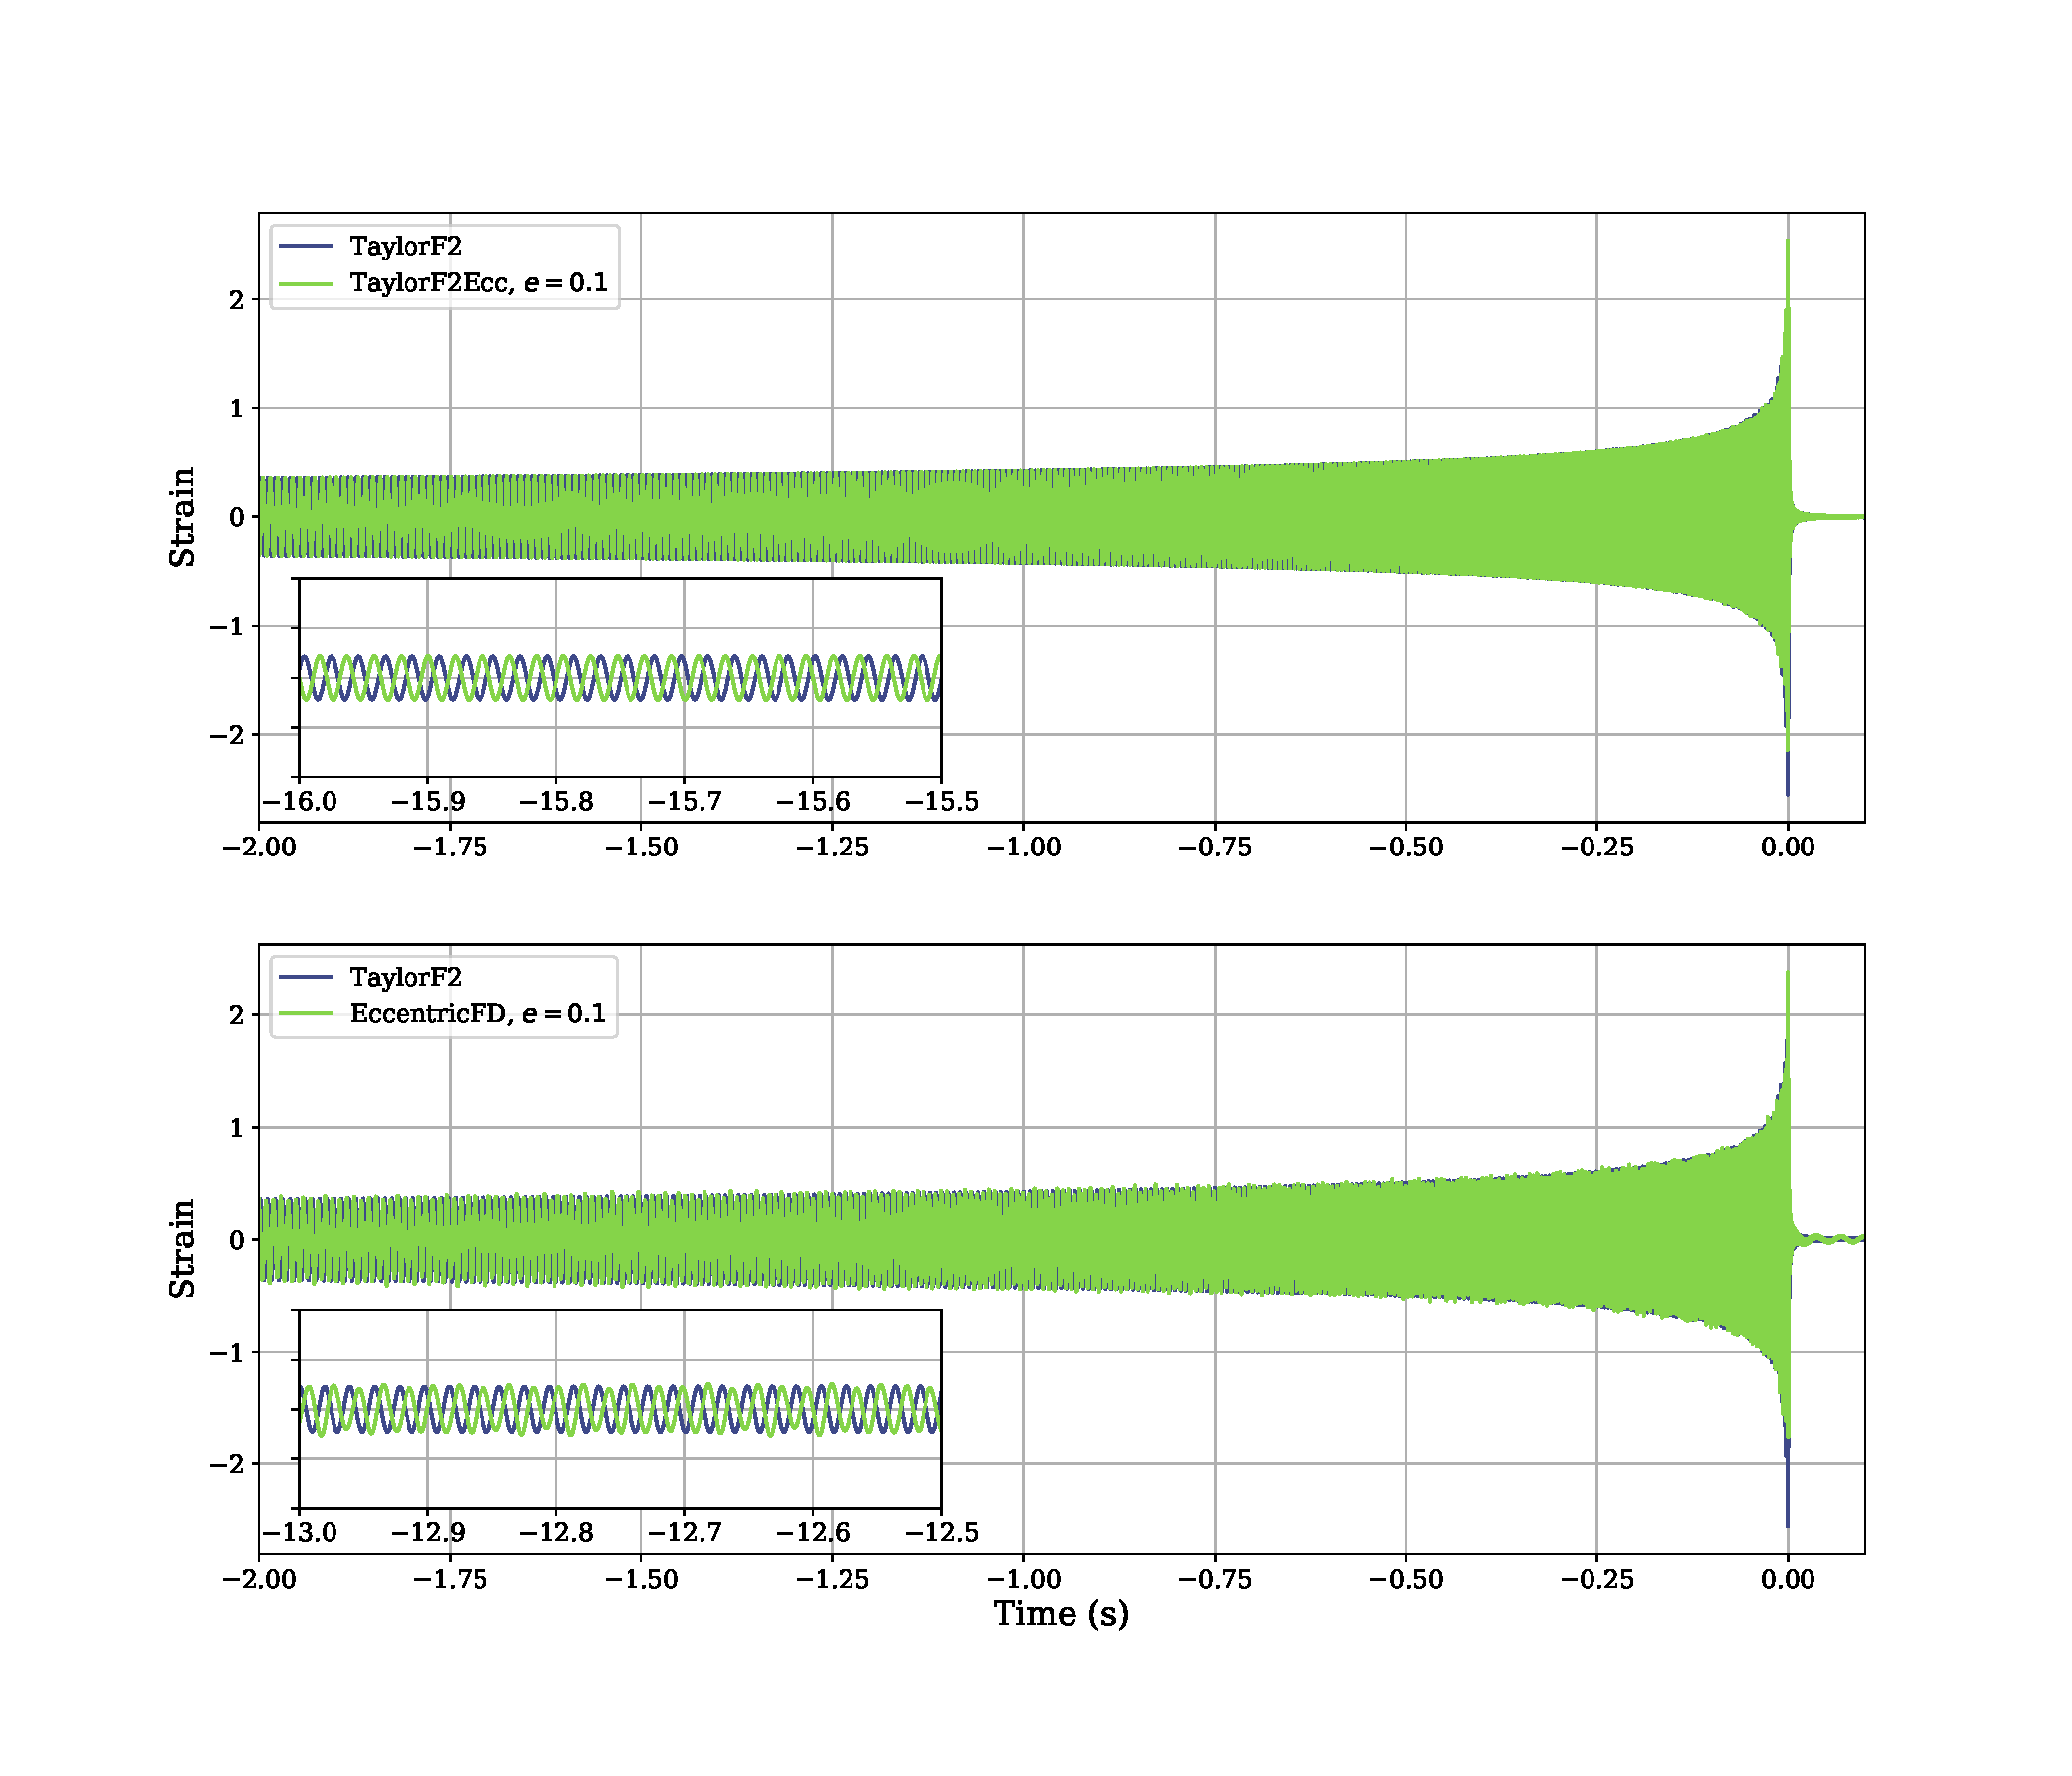
\includegraphics[width=1.0\textwidth,keepaspectratio]{Figures/Methods/Waveformplot.pdf}
    \caption{The scaled strain as a function of time for two eccentric gravitational waveform models. TaylorF2Ecc (top) EccentricFD (bottom) gravitational waveforms generated at a dominant-mode gravitational-wave reference frequency of 10Hz with component masses of 1.4$\msun$ at an eccentricity of $e=0.1$ compared with the non-eccentric TaylorF2 waveform that show merging binary neutron stars up to the time of merger. The inset plot shows a zoomed-in depiction of the the phase difference in the non-eccentric (violet) and eccentric (green) waveforms.}
    \label{fig:waveforms}
\end{figure}